\documentclass[pdf,xcolor={dvipsnames}]{beamer}
\usepackage{xcolor,soul}

\mode<presentation>{\usetheme{default}}
\title{An Efficient Exact Solution to the \newline ($l$,$d$) Planted Motif Problem}
\author{Maria Clara Isabel Sia*\\Julieta Nabos\\Proceso Fernandez}

\begin{document}
\begin{frame}\titlepage\end{frame}

\begin{frame}{Introduction}{The ($l,d$) planted motif problem}	
	\only<1>{
	\begin{itemize}
	\item {\color{red}motifs}: repeated, biologically significant subsequences in DNA \\\ \\
	\item {\color{red}DNA motif finding} must allow for mismatches due to mutation\\\ \\
	\item known as a difficult problem in computational biology and CS ({\color{red}NP-complete})\\\ \\
	\end{itemize}
	}

	\only<2>{\centering
	\emph{Find a motif of length {\color{red}$l$=8} across these 5 DNA sequences.}\\
	\emph{Each contains the motif with at most {\color{red}$d$=2} mismatches.}\\\ \\
	\small
	$S_1$\ \ \  \texttt{at{\color{red}cactcgtt}ctcctctaatgtgtaaagacgtactaccgacctta}\\\ \\
	$S_2$\ \ \  \texttt{acgccgaccggtc{\color{red}cgatcctt}gtatagctcctaacgggcatcagc}\\\ \\
	$S_3$\ \ \  \texttt{tcctgactgcatcgcgatctcggtagtttcctgt{\color{red}tcatcatt}ttt}\\\ \\
	$S_4$\ \ \  \texttt{ggccctca{\color{red}gcatcgtg}cgtcctgctaacacattcccatgcagctt}\\\ \\
	$S_5$\ \ \  \texttt{tgaaaagaatttacggtaaaggatccacatc{\color{red}caatcgtg}tgaaag}\\\ \\\ \\
	\emph{Planted motif: }\texttt{\color{red}ccatcgtt}\\
	}
	\end{frame}

\begin{frame}{Introduction}{Key concepts}
	\begin{itemize}
		\item $l$-mer
		\item Hamming distance $d_H$
		\item $d$-neighbor
		\end{itemize}
	\end{frame}

\begin{frame}{EMS-GT}{Introduction}
	\begin{itemize}
		\item an {\color{red}exact motif search} (EMS) algorithm that uses the 
		candidate {\color{red}generate-and-test} (GT) approach\\\ \\
		\item exact algorithms {\color{red}search exhaustively} to find all possible motifs,\\
		\begin{itemize}
			\item as opposed to heuristic ones which sample/guess motifs\\\ \\
			\end{itemize}
		\item {\em generate} - narrows the search to a {\color{red}set of candidate motifs}\\
		{\em test} - {\color{red}checks each candidate} to see if it is a motif
		\end{itemize}
	\end{frame}

\begin{frame}{EMS-GT}{Demonstration}
	\only<1>{\centering\small\ \\\ \\
	$S_1$\ \ \  \texttt{atcactcgttctcctctaatgtgtaaagacgtactaccgacctta}\\\ \\\ \\
	$S_2$\ \ \  \texttt{acgccgaccggtccgatccttgtatagctcctaacgggcatcagc}\\\ \\\ \\
	$S_3$\ \ \  \texttt{tcctgactgcatcgcgatctcggtagtttcctgttcatcattttt}\\\ \\\ \\\ \\
	$S_4$\ \ \  \texttt{ggccctcagcatcgtgcgtcctgctaacacattcccatgcagctt}\\\ \\\ \\
	$S_5$\ \ \  \texttt{tgaaaagaatttacggtaaaggatccacatccaatcgtgtgaaag}
	}
	\end{frame}

\begin{frame}{EMS-GT}{Representing sets}
	\only<1>{
	\begin{itemize}
		\item EMS-GT must operate on sets of $l$-mers.\\\ \\
		\item There are $4^l$ possible $l$-mers that can be formed with \{\texttt{a},\texttt{c},\texttt{g},\texttt{t}\}\\\ \\
		\item Thus, {\color{red}to represent a set of $l$-mers, EMS-GT uses $4^l$ bits},
			\begin{itemize}
				\item set to 1 if the corresponding $l$-mer is a member of the set,
				\item set to 0 otherwise.
				\end{itemize}\ \\\ \\
		\item For efficiency, EMS-GT stores the $4^l$ bits as {\color{red}$\frac{4^l}{32}$ 32-bit integers}.
		\end{itemize}
		}
	\only<2->{
	\begin{itemize}
			\item $N$(\ \texttt{acgt}, 1\ )\ \ \ \ $l$=4;\ \ $4^l$ = 256, $\frac{4^l}{32}$ = 8
		\end{itemize}\ \\
	}
	\only<2>{ \centering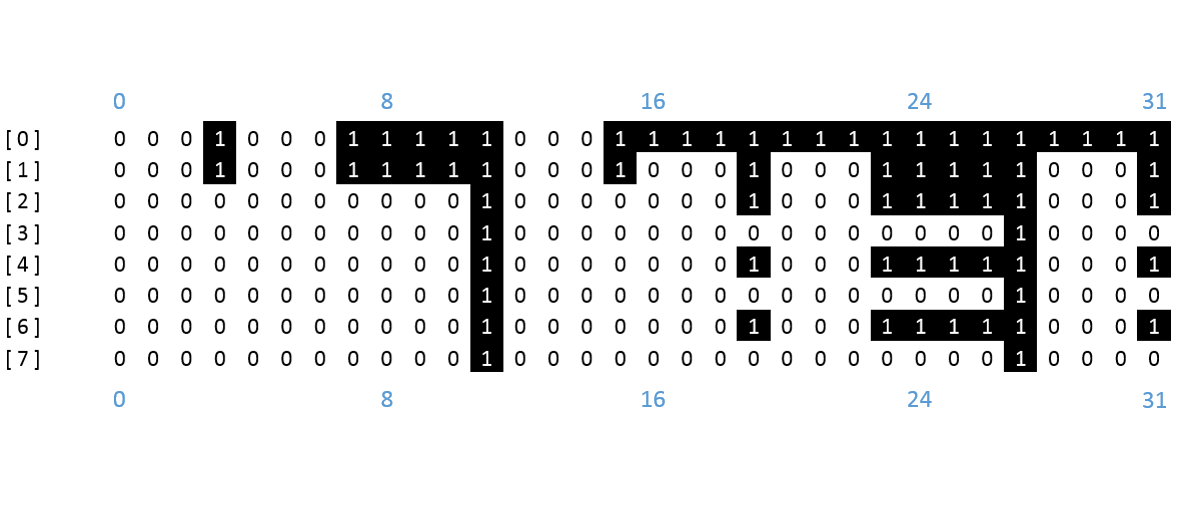
\includegraphics[width=\textwidth]{img/acgt1.png}\\ }
	\only<3>{ \centering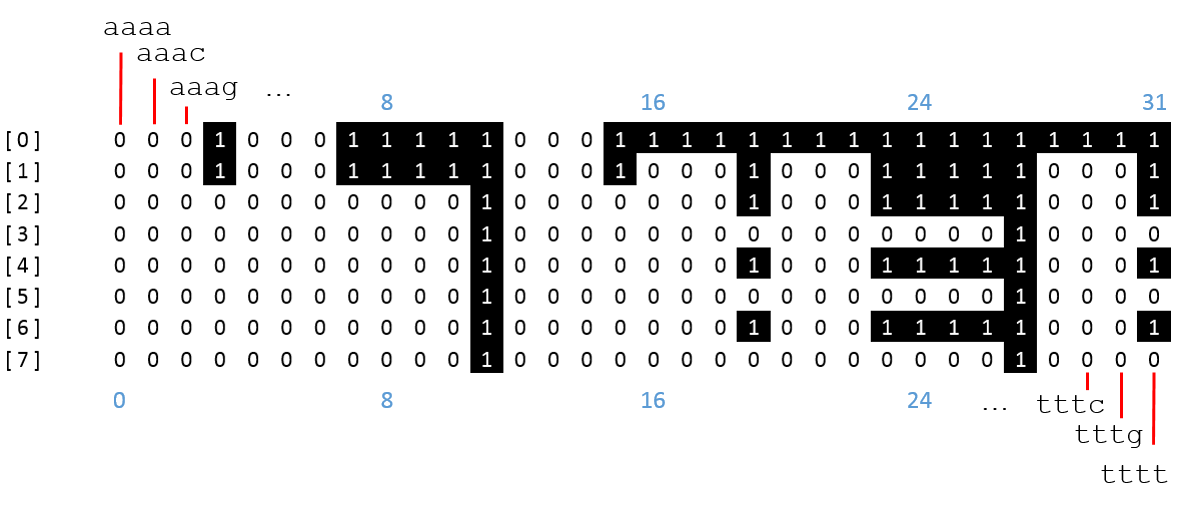
\includegraphics[width=\textwidth]{img/acgt2.png}\\ }
	\only<4>{ \centering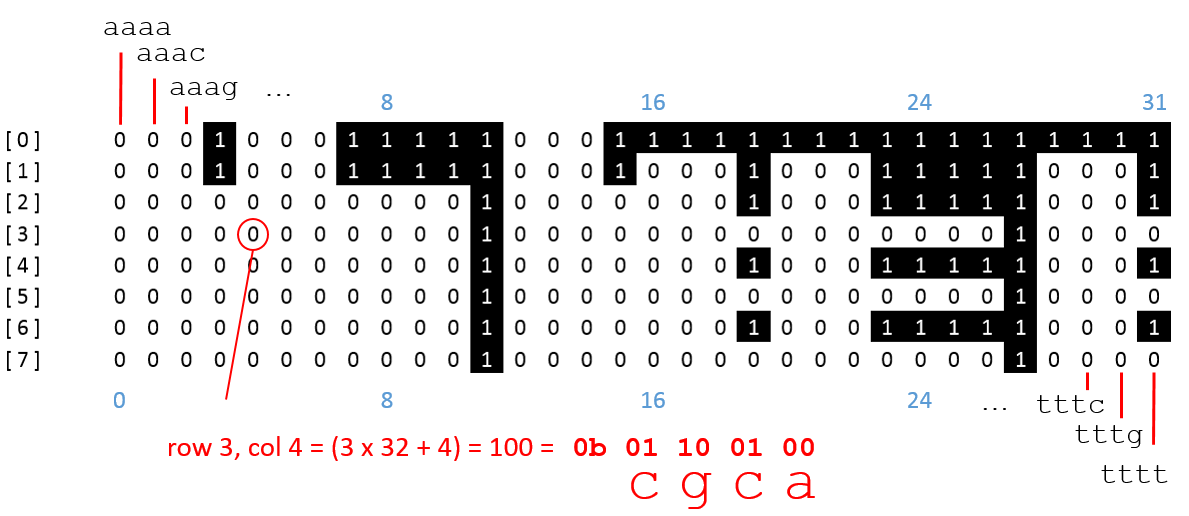
\includegraphics[width=\textwidth]{img/acgt3.png}\\ }
	\end{frame}

\begin{frame}{EMS-GT}{Building sets}
	discuss recursive
	\end{frame}

\begin{frame}{EMS-GT}{Building sets in blocks}
	
	\end{frame}

\begin{frame}{EMS-GT}{Results}

	\end{frame}

\end{document}